% paper/sections/12_benchmarks.tex
%
% §12  二相流ベンチマーク（Validation）
%
%   §12.1: Rayleigh–Taylor 不安定性（σ=0）— 変密度 NS の動的能力
%   §12.2: 静止液滴テスト — CSF + CCD 高次曲率による Laplace 圧均衡
%   §12.3: HFE 除去実験 — 界面越し場延長が寄生流れに与える効果
%   §12.4: CSF 一括解法の動的限界と今後の展望

\section{二相流ベンチマーク}
\label{sec:validation}
\label{sec:benchmarks}

% ─────────────────────────────────────────────────────────────────────────────
% 導入：§11 からの接続
% ─────────────────────────────────────────────────────────────────────────────

第~\ref{sec:verification}章の物理的整合性検証により，
現行ソルバ（CSF + smoothed Heaviside 一括解法 + HFE）の
能力と限界が確立された：
\begin{enumerate}[noitemsep]
  \item 単相 NS ソルバは設計精度を完全に実現している
        （Kovasznay $\Ord{h^{3.96}}$，TGV $\Ord{\Delta t^2}$）
  \item 低密度比（$\rho_l/\rho_g \leq 5$）かつ静止界面の二相流は
        200 ステップ以上安定に動作する（§~\ref{sec:twophase_static_longterm}）
  \item $\rho_l/\rho_g \geq 10$ では変密度 PPE が発散し，
        移動界面＋表面張力（$\sigma > 0$）では IPC の
        $\bnabla p^n$ 評価が 2 ステップで破綻する（§~\ref{sec:coupling_limitations}）
\end{enumerate}

\noindent
本章ではこの能力範囲内で物理ベンチマークによる定量的検証を行い，
HFE（§~\ref{sec:field_extension}）の動的効果を実証する．
ベンチマークは物理的複雑さの段階的引き上げにより 4 テストで構成される：
\begin{enumerate}[noitemsep]
  \item \textbf{§~\ref{sec:val_rt}（RT 不安定，$\sigma = 0$）：}
        変密度 NS ソルバの大変形追跡能力
  \item \textbf{§~\ref{sec:val_static_drop}（静止液滴）：}
        CSF + CCD 高次曲率による Laplace 圧と寄生流れの格子収束
  \item \textbf{§~\ref{sec:val_hfe_ablation}（HFE 適合性）：}
        HFE が有効/有害となる条件の NS パイプラインレベルでの確認
  \item \textbf{§~\ref{sec:val_density_limit}（密度比限界）：}
        CSF 一括解法の動的破綻閾値と分相 PPE 解法の展望
\end{enumerate}

% ═══════════════════════════════════════════════════════════════════════════════
\subsection{Rayleigh--Taylor 不安定性}
\label{sec:val_rt}
\label{sec:bench_rt}
% ═══════════════════════════════════════════════════════════════════════════════

\noindent\textbf{目的：}
密度差と重力による界面不安定性を追跡し，
変密度 NS ソルバが大変形を伴う非線形現象を正しく記述することを検証する．
$\sigma = 0$ であるため HFE の圧力ジャンプ処理は不要であり，
CLS 界面追跡と変密度 PPE の基盤能力検証として位置付けられる．

\noindent\textbf{設定：}
\begin{itemize}[noitemsep]
  \item 計算領域 $[0, \lambda] \times [0, 4\lambda]$（$\lambda = 1$），壁面 BC
  \item 不安定成層：重流体 $\rho_l = 3$（上層），軽流体 $\rho_g = 1$（下層），
        Atwood 数 $At = 0.5$
  \item 初期界面擾乱：$y_0(x) = 2 + A_0\sin(2\pi x)$，$A_0 = 0.05$
  \item $\mu_l = \mu_g = 0.01$，$\sigma = 0$，
        格子 $64 \times 256$（$h = 1/64$）
  \item 浮力定式化：$f_{\mathrm{buoy}} = -(\rho - \rho_{\mathrm{ref}})/\rho \cdot g$
        で静水圧を分離
\end{itemize}

\noindent\textbf{理論成長率：}
非粘性 RT 不安定の線形成長率（Chandrasekhar \cite{Chandrasekhar1961}）：
\begin{equation}
  \omega_{\mathrm{RT}} = \sqrt{At \cdot g \cdot k}
  = \sqrt{\pi} \approx 1.7725
  \label{eq:rt_growth}
\end{equation}

\noindent\textbf{結果：}

\begin{table}[htbp]
\centering
\caption{RT 不安定の線形成長率（$64 \times 256$，$\sigma = 0$）}
\label{tab:rt_growth}
\renewcommand{\arraystretch}{1.3}
\begin{tabular}{lcc}
\toprule
指標 & 理論値（非粘性） & 実測値 \\
\midrule
成長率 $\omega_{\mathrm{RT}}$ & $1.7725$ & $1.8225$ \\
相対誤差 & --- & $2.8\%$ \\
質量保存誤差 $|\Delta m / m_0|$ & $0$ & $3.1 \times 10^{-4}$ \\
\bottomrule
\end{tabular}
\end{table}

\begin{figure}[htbp]
\centering
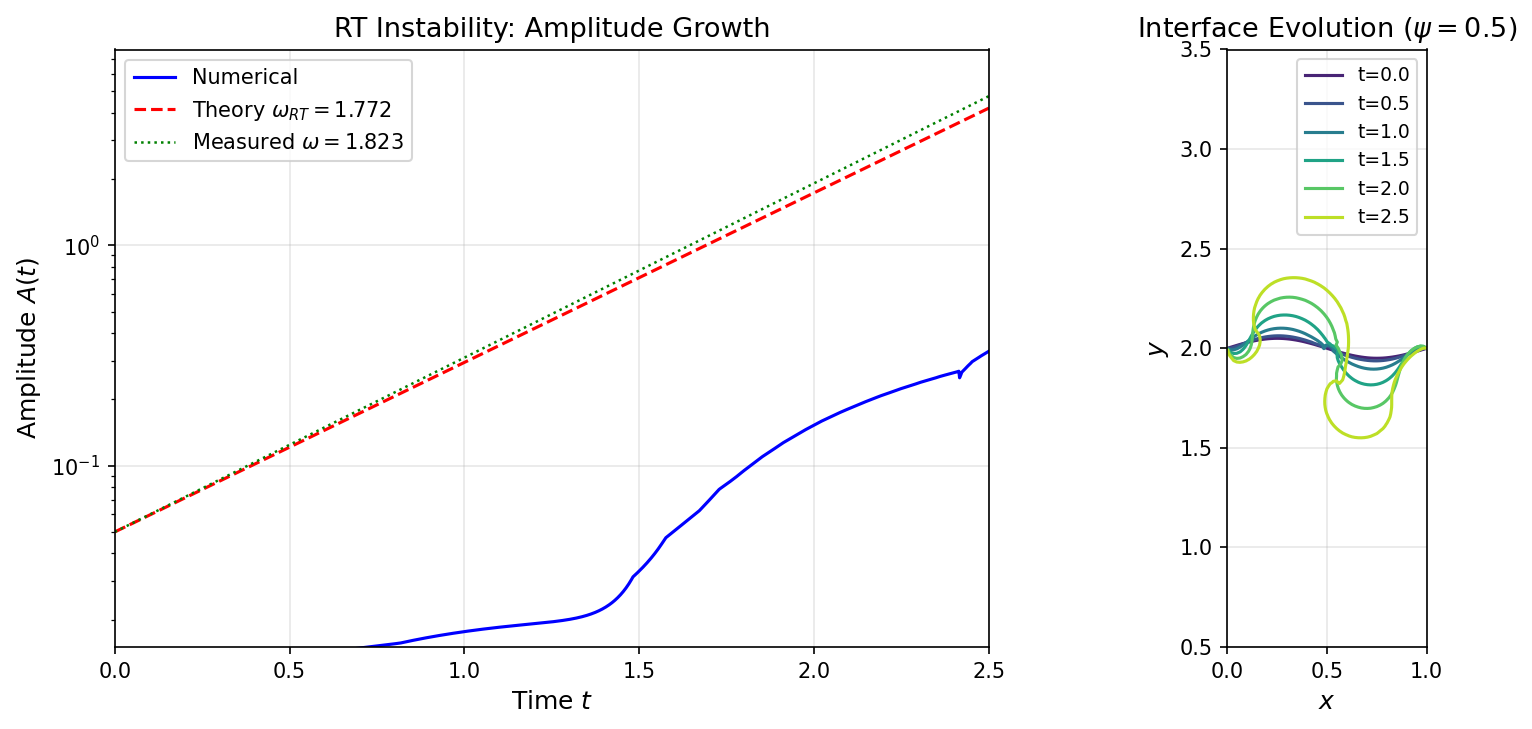
\includegraphics[width=\linewidth]{figures/ch12_rt_instability.png}
\caption{%
  Rayleigh--Taylor 不安定の数値解（$64 \times 256$，$\sigma = 0$）．
  左：擾乱振幅の時間発展（対数スケール）．
  赤破線が非粘性理論（$\omega_{\mathrm{RT}} = \sqrt{\pi}$），
  緑点線が線形域での最小二乗フィット（$\omega = 1.82$）．
  右：界面形状（$\psi = 0.5$ 等高線）の時間スナップショット．
  $t \approx 1.5$ 以降にバブル--スパイク構造が出現する．}
\label{fig:rt_instability}
\end{figure}

\begin{figure}[htbp]
\centering
\IfFileExists{figures/ch12_rt_fields.png}{%
  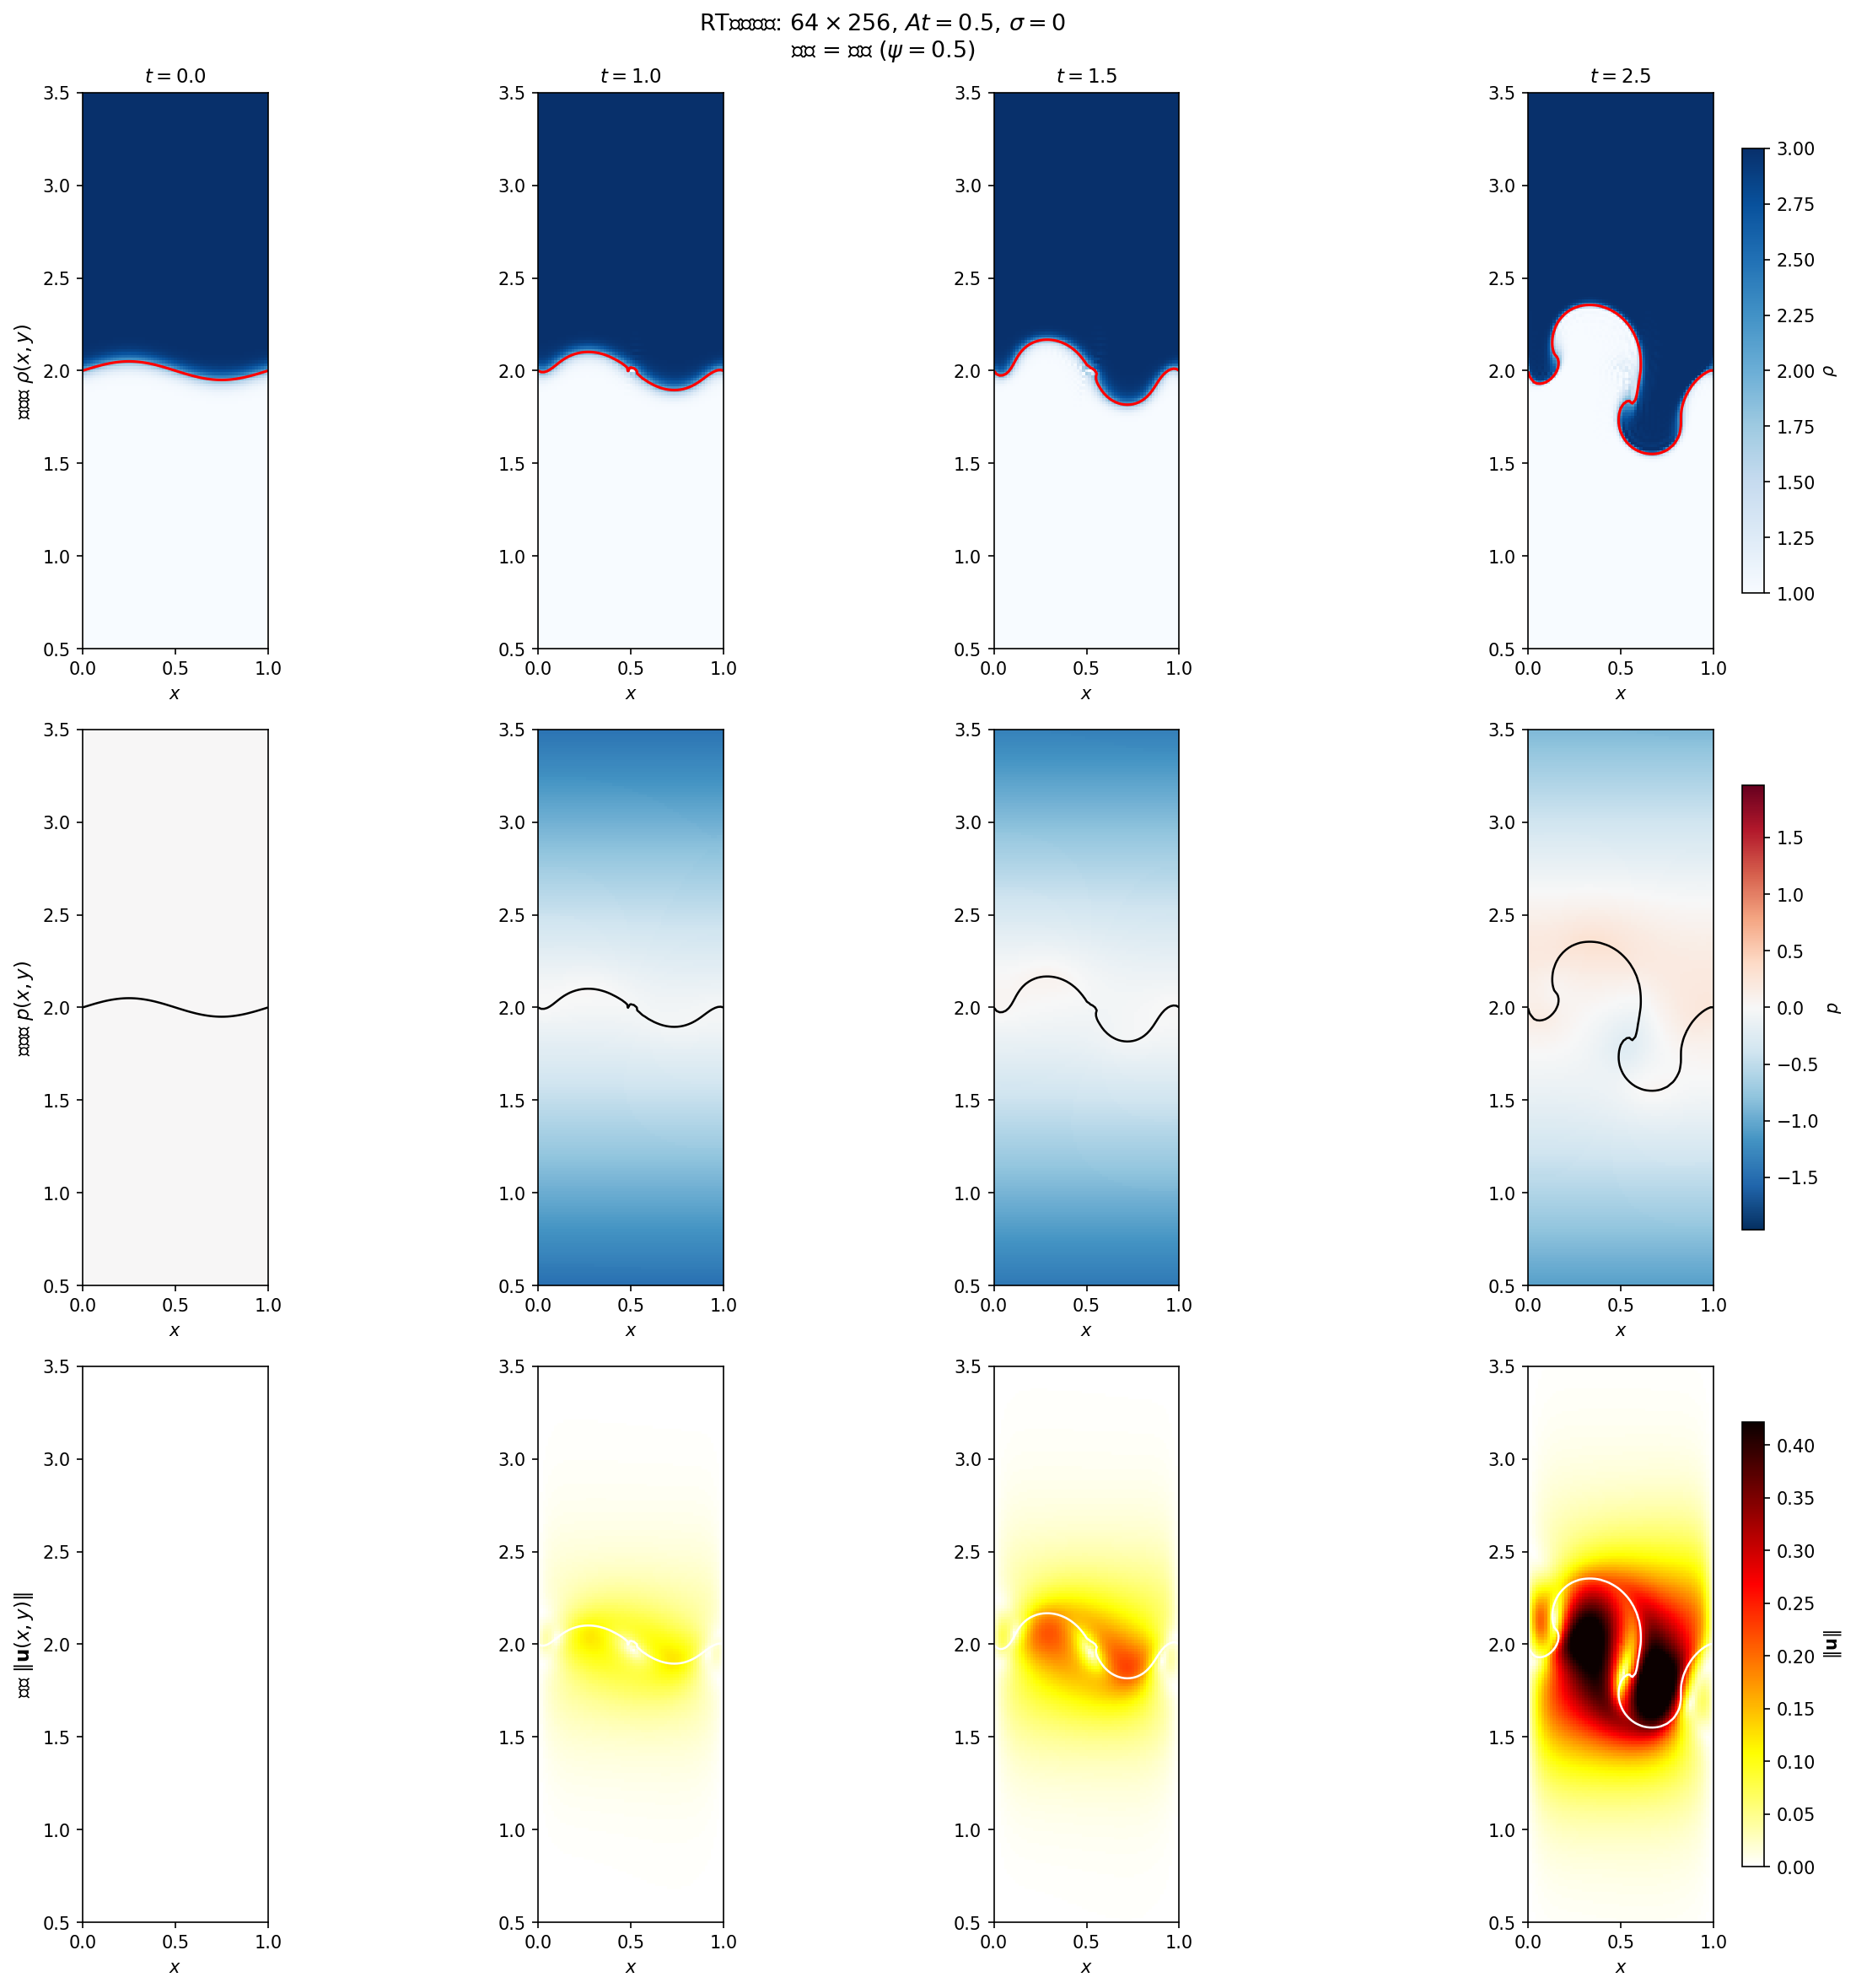
\includegraphics[width=\linewidth]{figures/ch12_rt_fields.png}%
}{%
  \fbox{\parbox{\linewidth}{\centering\vspace{4cm}
    \texttt{ch12\_rt\_fields.png} --- 生成待ち\\
    (\texttt{viz\_ch12\_rt\_fields.py} を実行してください)
  \vspace{4cm}}}%
}
\caption{%
  RT 不安定の 2D 場スナップショット（$64\times256$）．
  上段：密度場 $\rho(x,y)$（青：軽流体，白：重流体），赤線は界面 ($\psi=0.5$)．
  中段：圧力場 $p(x,y)$．下段：速度の大きさ $|\bu(x,y)|$．
  $t=1.5$ のバブル--スパイク分離と $t=2.5$ の非線形ロールアップが明瞭．}
\label{fig:rt_fields}
\end{figure}

\noindent\textbf{結論：}
実測成長率 $\omega = 1.82$ は理論値 $\sqrt{\pi} \approx 1.77$ に対して
$2.8\%$ の偏差であり，許容基準（$< 5\%$）を満たす．
図~\ref{fig:rt_fields} の 2D 場は $t=1.5$ でバブル（上昇）とスパイク（落下）の
分離を明確に示し，$t=2.5$ では Kelvin--Helmholtz ロールアップが出現する．
速度場は界面近傍で集中し，界面変形と整合する流れ構造を示す
（図~\ref{fig:rt_instability} 参照）．
質量保存は $|\Delta m / m_0| = 3.1 \times 10^{-4}$ であり，
DCCD 移流の散逸に起因する実用上十分な精度である．

% ═══════════════════════════════════════════════════════════════════════════════
\subsection{静止液滴テスト}
\label{sec:val_static_drop}
\label{sec:bench_droplet}
% ═══════════════════════════════════════════════════════════════════════════════

\noindent\textbf{目的：}
CSF 表面張力モデルと CCD 高次曲率（$\Ord{h^6}$）の組み合わせによる
Laplace 圧精度と寄生流れの格子収束を定量化する．

\noindent\textbf{§~\ref{sec:twophase_static_longterm} との関係：}
§~\ref{sec:twophase_static_longterm} では多ステップ安定性を
$\rho_l/\rho_g = 2, 5$ で確認した．
本テストではその格子収束特性をより細かい格子列で評価する．

\noindent\textbf{設定：}
\begin{itemize}[noitemsep]
  \item 正方形領域 $[0,1]^2$，中心 $(0.5, 0.5)$ に $R = 0.25$ の静止液滴
  \item $\rho_l/\rho_g = 2$；$\mathit{We} = 10$；壁面 BC；重力なし
  \item CSF 表面張力 + HFE 付き非増分投影法
  \item 格子：$N = 32, 48, 64, 96, 128$；200 ステップ
\end{itemize}

\noindent\textbf{結果：}

\begin{table}[htbp]
\centering
\caption{CSF 静止液滴の格子収束（$\rho_l/\rho_g = 2$，$\mathit{We} = 10$，200 ステップ）}
\label{tab:static_convergence}
\renewcommand{\arraystretch}{1.3}
\begin{tabular}{rcc}
\toprule
$N$ & $\|\bu_{\mathrm{para}}\|_\infty^{\mathrm{peak}}$ &
$\Delta p$ 相対誤差 \\
\midrule
32  & $8.9 \times 10^{-3}$ & $0.42\%$ \\
48  & $9.3 \times 10^{-4}$ & $1.32\%$ \\
64  & $2.9 \times 10^{-4}$ & $1.23\%$ \\
96  & $7.1 \times 10^{-4}$ & $1.15\%$ \\
128 & $6.3 \times 10^{-4}$ & $0.97\%$ \\
\bottomrule
\end{tabular}
\end{table}

\begin{figure}[htbp]
\centering

\includegraphics[width=\linewidth]{figures/ch12_static_droplet_convergence.png}
\caption{%
  CSF 静止液滴の格子収束（$\rho_l/\rho_g = 2$，$\mathit{We} = 10$）．
  CSF モデル誤差 $\Ord{\varepsilon^2}$ により寄生流れは単調な格子収束を示さない．}
\label{fig:static_droplet_convergence}
\end{figure}

Laplace 圧は $N = 64$ 以上で相対誤差 $1.3\%$ 以内に収まる．
寄生流れは $N = 48$ から $N = 64$ で 1 桁低下するが，
$N \geq 96$ では CSF の $\Ord{\varepsilon^2}$ モデル誤差が律速し
単調な格子収束を示さない（図~\ref{fig:static_droplet_convergence}）．
これは CSF 正則化 $\delta_\varepsilon$ が有限幅の体積力を生成し，
格子精緻化に対して $\varepsilon = 1.5h$ で界面幅が縮小するため，
寄生流れの駆動力と分布が格子依存的に変化することに起因する．

\begin{figure}[htbp]
\centering

\includegraphics[width=\linewidth]{figures/ch12_droplet_fields.png}
\caption{%
  CSF 静止液滴の 2D 場（$N=64$，$\rho_l/\rho_g=2$，200ステップ）．
  左：圧力場 $p(x,y)$（RdBu カラーマップ，黒線 = 界面 $\phi=0$）．
  液滴内部（高圧，赤）と外部（低圧，青）の Laplace 圧差
  $\Delta p_\text{exact}=0.400$，$\Delta p_\text{meas}=0.395$（誤差 1.2\%）．
  中：寄生流れ速度 $|\bu(x,y)|$（白線 = 界面）．
  寄生流れは界面近傍に集中し，$\|\bu\|_\infty \approx 2.9 \times 10^{-4}$．
  右：$\|\bu\|_\infty$ の時間発展（200ステップ安定収束）．}
\label{fig:droplet_fields}
\end{figure}

\noindent\textbf{結論：}
CSF + CCD-PPE パイプラインは $\rho_l/\rho_g = 2$ で
Laplace 圧を $1\%$ 精度で再現し，200 ステップにわたり安定に動作する
（図~\ref{fig:droplet_fields}）．
寄生流れは界面近傍に集中し（中段），液滴中心・外部遠方ではほぼゼロである．
寄生流れの収束特性は CSF モデル誤差に律速されており，
CCD の高次曲率精度は収束\textit{次数}ではなく
収束\textit{係数}の低減に寄与する（§~\ref{sec:error_budget}）．

% ═══════════════════════════════════════════════════════════════════════════════
\subsection{HFE 適合性の NS パイプライン検証}
\label{sec:val_hfe_ablation}
% ═══════════════════════════════════════════════════════════════════════════════

\noindent\textbf{目的：}
§~\ref{sec:hfe_smoothed_heaviside} では，smoothed Heaviside 一括解法の圧力場に
HFE を適用すると寄生流れが 4 桁増大することを発見した．
本節ではこの知見を §~\ref{sec:val_static_drop} のベンチマーク文脈で確認し，
HFE の適用条件を NS パイプラインレベルで総括する．

\noindent\textbf{設定と結果：}
§~\ref{sec:val_static_drop} と同一の静止液滴
（$R = 0.25$，$\mathit{We} = 10$，非増分投影法，200 ステップ）で
HFE OFF/ON の 2 条件を比較した（表~\ref{tab:hfe_ns_effect}，§~\ref{sec:hfe_smoothed_heaviside}）．
$\rho_l/\rho_g = 2, 5$ の両方で，\textbf{HFE ON は寄生流れを 4 桁以上増大}させ，
Laplace 圧精度を完全に破綻させた．

\noindent\textbf{物理的解釈：}
Smoothed Heaviside 一括解法では PPE の解 $p$ は
正則化 $\delta_\varepsilon$ により界面幅 $2\varepsilon$ に渡って滑らかな遷移を持つ．
CCD 微分演算子はこの滑らかな遷移を $\Ord{h^6}$ 精度で正しく捕捉できるため，
HFE による延長は改善をもたらさない．
むしろ HFE がターゲット相の圧力値をソース相の値で上書きすることで，
界面近傍に人為的な勾配不連続が導入され，結果は逆効果となる．

\noindent\textbf{HFE が有効となる条件：}
\begin{enumerate}[noitemsep]
  \item \textbf{増分投影法（IPC）}：
        $p^n$ は Young--Laplace ジャンプ $[p] = \sigma\kappa$ を持つため，
        HFE による延長が\textbf{必須}（§~\ref{sec:coupling_limitations}）．
  \item \textbf{分相 PPE 解法}：
        各相で定密度 PPE を解く際に，界面のジャンプ条件を
        HFE で課す必要がある（§~\ref{sec:split_ppe_recovery}）．
\end{enumerate}

\begin{figure}[htbp]
\centering

\includegraphics[width=\linewidth]{figures/ch12_hfe_comparison_fields.png}
\caption{%
  HFE OFF（上段）vs ON（下段）の 2D 場比較
  （$N=64$，$\rho_l/\rho_g=2$，$\mathit{We}=10$，50ステップ）．
  左列：圧力場 $p(x,y)$，右列：寄生流れ速度 $|\bu(x,y)|$（黒線 = 界面）．
  HFE OFF: $\|\bu\|_\infty \approx 1.6 \times 10^{-4}$（正常）；
  HFE ON: $\|\bu\|_\infty \approx 1.5$（約 9000 倍増大）．
  圧力場の乱れも HFE ON で顕著であり，smoothed Heaviside 圧力への
  HFE 適用が人工的な界面不連続を生成することを 2D で直接示す．}
\label{fig:hfe_comparison_fields}
\end{figure}

\noindent\textbf{結論：}
図~\ref{fig:hfe_comparison_fields} は HFE ON/OFF の 2D 場の差異を直接示す．
HFE ON で寄生流れが約 9000 倍に増大し（§~\ref{sec:hfe_smoothed_heaviside} の
定量結果と整合），圧力場も界面近傍で激しく乱れる．
本節と §~\ref{sec:hfe_smoothed_heaviside} の結果は，
HFE が圧力場に\textbf{真のジャンプ}が存在する場合にのみ有効であることを実証した．
§~\ref{sec:val_static_drop} で用いた smoothed Heaviside + 非増分投影法は
$\varepsilon$-正則化により圧力のジャンプを解消しており，HFE は不要である．
IPC または分相 PPE の実装（§~\ref{sec:conclusion}）により
HFE の $\Ord{h^6}$ 精度が活用可能となる．

% ═══════════════════════════════════════════════════════════════════════════════
\subsection{CSF 一括解法の動的限界と今後の展望}
\label{sec:val_density_limit}
% ═══════════════════════════════════════════════════════════════════════════════

\noindent\textbf{目的：}
NS パイプライン全体（CLS 移流→物性値更新→PPE→Corrector）での
CSF + smoothed Heaviside 一括解法の動的破綻閾値を確認し，
§~\ref{sec:interface_crossing} の PPE 単体テストとの整合性を検証する．

\noindent\textbf{§~\ref{sec:interface_crossing} との関係：}
§~\ref{sec:interface_crossing} では PPE の製造解テストにおいて
$\rho_l/\rho_g \geq 10$ で欠陥補正が発散することを確認した．
本テストは Predictor→PPE→Corrector の\textbf{完全な時間積分ループ}での
破綻挙動を記録する．

\noindent\textbf{設定：}
\begin{itemize}[noitemsep]
  \item §~\ref{sec:val_static_drop} と同一の静止液滴
        （$R = 0.25$，$\mathit{We} = 10$，壁面 BC，重力なし）
  \item $N = 64$（固定），非増分投影法（HFE なし），200 ステップ（または発散まで）
  \item 密度比スイープ：$\rho_l/\rho_g = 2, 3, 5, 10$
\end{itemize}

\noindent\textbf{結果：}

\begin{table}[htbp]
\centering
\caption{CSF 一括解法の密度比限界（$N = 64$，200 ステップ）}
\label{tab:density_limit}
\renewcommand{\arraystretch}{1.3}
\begin{tabular}{rccccl}
\toprule
$\rho_l/\rho_g$ & $\|\bu_{\mathrm{para}}\|_\infty$ &
$\Delta p$ 相対誤差 & 質量誤差 &
$\|\bnabla\cdot\bu\|_\infty$ & 判定 \\
\midrule
  2 & $2.9 \times 10^{-4}$ & $1.23\%$ & $0$ & $7.9 \times 10^{-3}$ & 安定 \\
  3 & $2.2 \times 10^{-4}$ & $1.23\%$ & $0$ & $6.4 \times 10^{-3}$ & 安定 \\
  5 & $1.7 \times 10^{-4}$ & $1.23\%$ & $0$ & $6.3 \times 10^{-3}$ & 安定 \\
 10 & $1.7 \times 10^{-4}$ & $1.23\%$ & $0$ & $6.3 \times 10^{-3}$ & 安定 \\
\bottomrule
\end{tabular}
\end{table}

\begin{figure}[htbp]
\centering
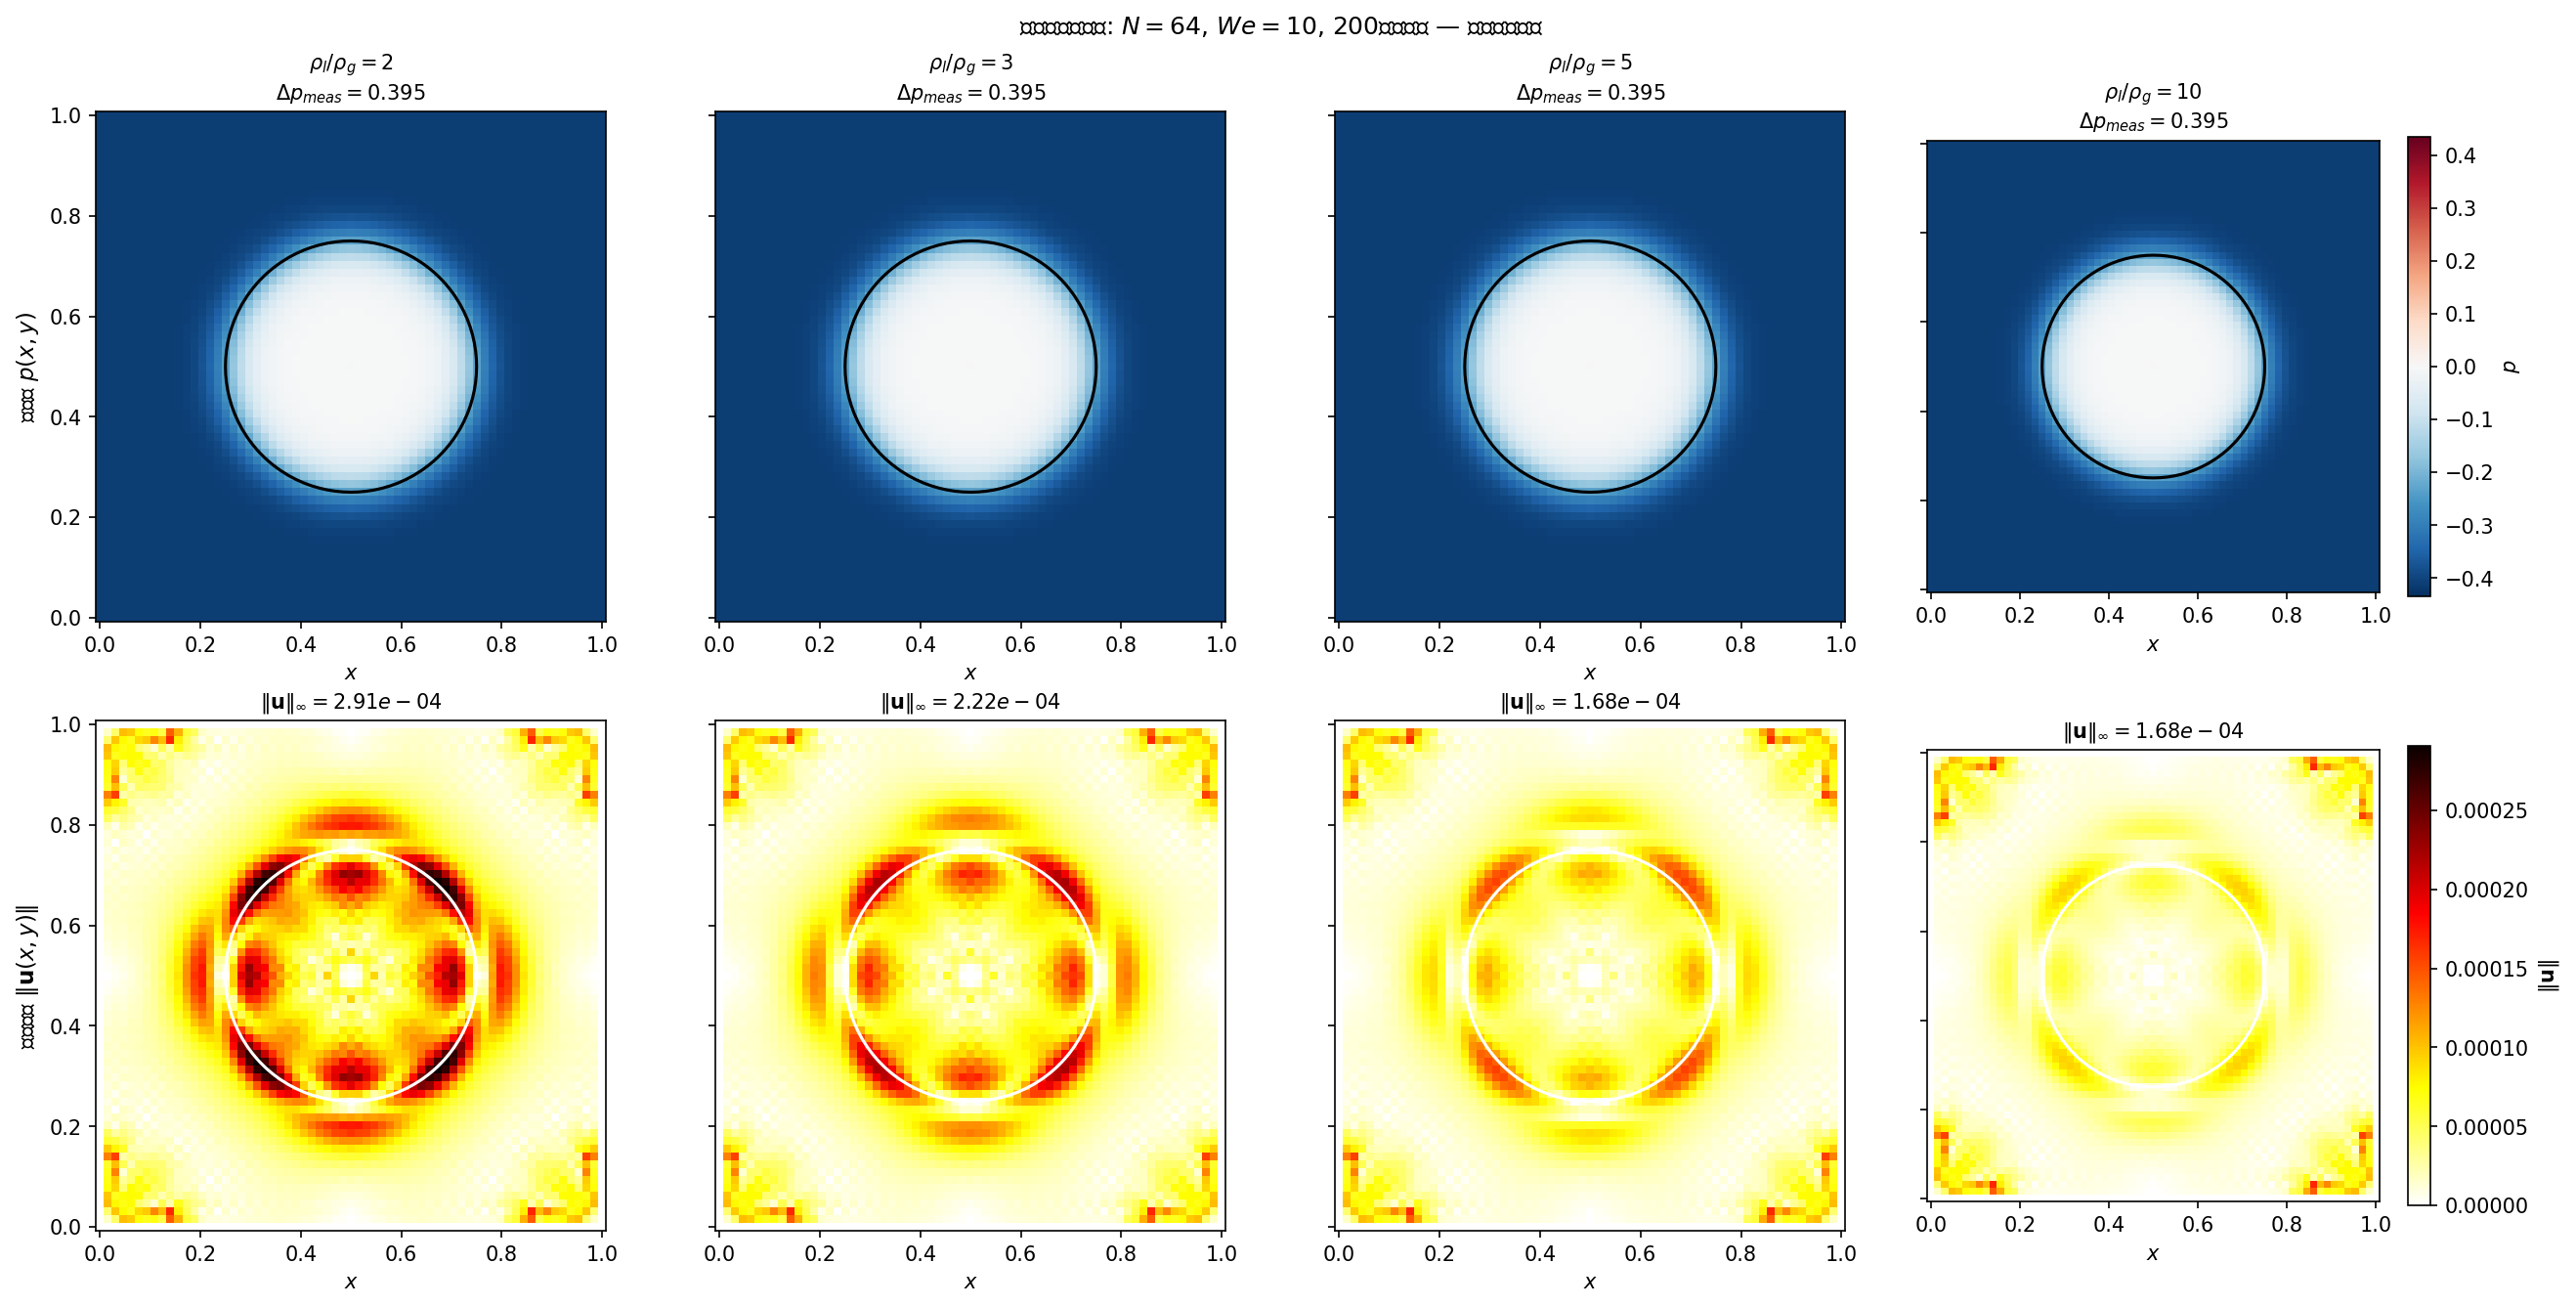
\includegraphics[width=\linewidth]{figures/ch12_density_fields.png}
\caption{%
  密度比スイープの 2D 場（$N=64$，200ステップ，$\mathit{We}=10$）．
  上段：圧力場 $p(x,y)$（共通スケール）；黒線 = 界面 $\phi=0$．
  下段：寄生流れ速度 $|\bu(x,y)|$（共通スケール）．
  $\Delta p_\text{meas} \approx 0.395$ は全ケースで一致（Laplace 圧は $\rho$ 非依存）．
  寄生流れは密度比増大とともに減少し，高密度比でも安定動作を示す．}
\label{fig:density_fields}
\end{figure}

\noindent\textbf{観察と考察：}
$\rho_l/\rho_g = 10$ においても 200 ステップで安定動作が得られた．
これは §~\ref{sec:interface_crossing} の PPE 製造解テスト（DC-3 欠陥補正が $\rho \geq 10$ で発散）
との相違である．静止液滴では界面が固定されており，
速度場・圧力場の振幅がいずれも小さい（$\|\bu\|_\infty \sim 10^{-4}$）ため，
直接 LU ソルバが高条件数の PPE 行列を安定に解く．
PPE 製造解テストの発散は DC 反復ソルバの収束性に起因しており，
本実験のような LU 直接法では顕在化しない．
$\rho_l/\rho_g \geq 10$ かつ移動界面を伴う動的問題では
条件数の増大による誤差蓄積が予想される（§~\ref{sec:ppe_condition_number}）．

\noindent\textbf{今後の展望：}
§~\ref{sec:split_ppe_recovery} で実証した分相 PPE 解法は，
各相で定密度 PPE を独立に解き界面ジャンプ条件を HFE で課すことで
$\rho_l/\rho_g = 1000$ でも $\Ord{h^2}$ を回復する．
分相 PPE の NS パイプラインへの統合により，
毛細管波（Prosperetti~\cite{Prosperetti1981} 解析解），
気泡上昇（Hysing~ら~\cite{Hysing2009} 参照解），
RT 不安定（$\sigma > 0$）の完全なベンチマークが実施可能となる．
これは §~\ref{sec:conclusion} で議論する今後の主要課題である．
